\documentclass[conference]{IEEEtran}
\IEEEoverridecommandlockouts
\usepackage{cite}
\usepackage{amsmath,amssymb,amsfonts}
\usepackage{algorithmic}
\usepackage{graphicx}
\usepackage{textcomp}
\usepackage{xcolor}
\bibliographystyle{IEEEtran}
\def\BibTeX{{\rm B\kern-.05em{\sc i\kern-.025em b}\kern-.08em
    T\kern-.1667em\lower.7ex\hbox{E}\kern-.125emX}}
% --- float placement limits: allow a bottom float to share a column with a top float
\renewcommand{\topfraction}{0.9}
\renewcommand{\bottomfraction}{0.6}
\renewcommand{\textfraction}{0.1}
\renewcommand{\floatpagefraction}{0.7}
\setcounter{topnumber}{2}
\setcounter{bottomnumber}{2}
\setcounter{totalnumber}{4}
% --- space reclaim: tightens float and display separation only. No font, margin,
% --- or line-spacing change, so it stays inside IEEE formatting rules.
% --- DELETE THIS BLOCK to restore stock spacing. Yield ~7 lines:
% --- 6 floats x ~10pt of float separation, 2 displayed equations x ~12pt.
\setlength{\textfloatsep}{10pt plus 2pt minus 2pt}
\setlength{\dbltextfloatsep}{10pt plus 2pt minus 2pt}
\setlength{\abovedisplayskip}{4pt plus 2pt minus 2pt}
\setlength{\belowdisplayskip}{4pt plus 2pt minus 2pt}
\setlength{\abovedisplayshortskip}{2pt plus 1pt}
\setlength{\belowdisplayshortskip}{2pt plus 1pt}
\renewcommand{\baselinestretch}{0.86}
\begin{document}
\title{SPRUCE: Pre-Prefill Compilation for Training-Free, Sublinear Per-Query Long-Context Retrieval
\thanks{SPRUCE is open source under Apache 2.0: \texttt{pip install sprucekit}. Code
and the evaluation harness are at \texttt{https://github.com/Rand0miz/spruce}.}}
\author{\IEEEauthorblockN{Myles McDaniel}
\IEEEauthorblockA{\textit{dept. name of organization (of Aff.)} \\
\textit{name of organization (of Aff.)}\\
City, Country \\
ORCID 0009-0003-7828-2343}
\and
\IEEEauthorblockN{Andreea Sistrunk}
\IEEEauthorblockA{\textit{dept. name of organization (of Aff.)} \\
\textit{name of organization (of Aff.)}\\
City, Country \\
ORCID 0000-0000-0000-0028}
}
\maketitle
\begin{abstract}
Long-context inference is usually treated as a model problem: the transformer can
read the whole prompt, so the task is to make that read cheaper. We introduce
\emph{context compilation}, a preprocessing paradigm in which a long prompt is
algorithmically transformed into a much smaller one before inference, leaving the
model untouched. On a sealed 288-prompt retrieval suite spanning 16K to 128K tokens, a frozen
Qwen2.5-Coder-1.5B-Instruct with static YaRN scaling answered only 66.7 percent
of questions correctly when given the entire document, and its accuracy fell as the
evidence moved farther from the final question. Our compiler, SPRUCE (Source-Preserving Recursive Untrained Compilation Engine), builds a
radix-2 hierarchy of Boolean lexical sketches over the tokenized prompt, descends it
with a fixed-width beam to locate a few source blocks, and returns those blocks to
their original text as a short document the same model reads with ordinary dense
attention. It consumes only tokenizer output, so it applies to any tokenizer-based
model without modification; nothing is trained and no text is paraphrased. On the same prompts the compiled path
scored 82.3 percent, a 15.6 point improvement with 63 compiler-only wins against 18
dense-only wins, and the gain was largest where dense reading was weakest: at the
shallowest evidence depth over 64K to 128K contexts, dense scored 40.0 percent
against 83.3 percent. Because the packet is sized by the selection budget rather than
the prompt, the model received a near-constant 1,850 tokens at every context length,
1.41 percent of the prompt at 128K. The request is therefore linear in context
length: it was faster at every length, from 2.49 to 14.08 times, and held peak
allocated GPU memory near 3.27 GB while dense grew from 4.66 GB to 15.58 GB.
\end{abstract}

\begin{IEEEkeywords}
context compilation, long-context language models, training-free
inference, pre-prefill selection, exact-text retrieval, frozen
backbone, sublinear per-query cost
\end{IEEEkeywords}

\section{Introduction}

A pretrained transformer extended to a long context window can, mechanically, see
every token of its prompt. Most work on long context follows from this: because
attention already reaches the evidence, the remaining problem is to make the read
cheaper. Such methods construct or learn a selector that identifies which blocks
matter, skip the rest, and are evaluated on how little quality they lose relative to
the dense model they approximate. The transformer stays in the critical path, and
dense attention is the ceiling.

Our measurements do not support that framing at the lengths where long-context
methods are actually deployed. On a sealed suite of 288 paired retrieval prompts,
a frozen Qwen2.5-Coder-1.5B-Instruct with static YaRN scaling to 131,072
positions answered 192 of 288 questions correctly when given the complete
document. Its accuracy was not uniform: it fell from 77.8 percent at 16K to
55.6 percent at 80K, and, more sharply, it fell with the distance between the
evidence and the final question. When the answer lay in the first tenth of the
document, dense reading was correct 47.9 percent of the time overall and
40.0 percent of the time at 64K and beyond. Dense access did not produce reliable
retrieval; irrelevant text, close lexical distractors, and positional distance
overwhelmed the relevant passage.

This reframes the objective. If dense attention were a ceiling, the best a selection
method could do is lose nothing. If it is instead degraded by the very length it is
asked to handle, then removing most of the document before the model reads it can be
more accurate than reading everything, not merely cheaper.

SPRUCE\footnote{Open
source under Apache 2.0: \texttt{pip install sprucekit}; code and evaluation harness
at \texttt{github.com/Rand0miz/spruce}.} is built on that
observation. It is a \emph{context compiler}: a training-free pass that runs before
the model's first forward pass, locates a small number of source regions, and hands
the model a short document made of their \emph{original, unmodified text}. It tokenizes the prompt with character
offsets, hashes token unigrams and adjacent token pairs into fixed-width Boolean
sketches over 64-token blocks, builds a radix-2 tree by Boolean union over children,
weights the question's hashed features by squared block inverse document frequency,
and descends the tree with a beam of 16 to return four source blocks. Those blocks
are expanded by one block on each side, repaired to paragraph boundaries, stitched
in source order, and re-encoded with ordinary dense attention. Because it consumes
only tokenizer output, it is independent of model architecture, weights and attention
implementation; nothing is trained and no text is paraphrased.

We contribute a measured argument that dense long-context reading is not a ceiling,
with the compiled path at 237/288 against dense 192/288 (exact McNemar
$p=5.20\times10^{-7}$) and an advantage that \emph{grows} with evidence-to-query
distance; a training-free compiler whose every cost fits inside the reported request
time while still beating dense at all eight lengths; a mechanism attribution
localizing residual error to evidence location rather than reading; and a cost
profile detached from context length, in which the model's input, prefill and KV
cache are all independent of $n$ and the request is linear in it.

\section{Background}

\subsection{Making the model's read cheaper}

The closest work attacks the same cost from inside the model, converting a
pretrained transformer into a sparse-attention model without retraining it. HiP
\cite{hip} performs a training-free greedy binary-tree search over key ranges,
scoring a representative token per range and keeping the global top-$k$ branches.
SeerAttention \cite{seer} trains a lightweight block gate by
self-distillation against the backbone's own pooled attention mass. SpotAttention
\cite{spot} trains a selector by KL distillation to estimate the full attention
distribution, reading a variable per-query budget from it. HISA \cite{hisa} replaces a flat indexer
with a two-stage coarse-then-fine search over pooled block representations.

Two properties are common to all four, and both separate them from compilation.
Selection happens \emph{inside} attention, so the model still ingests the entire
prompt and the selector only decides what a query may attend to. And dense attention
is the reference, with quality reported as preservation relative to it.

Both properties persist in the newest work, which optimizes the selector rather than
the attention it feeds: DeepSeek Sparse Attention \cite{dsa} learns a token-wise
indexer that scores every prefix token, and MISA \cite{misa} routes a
query-dependent subset of that indexer's heads to cut its cost without training,
MISA is measured against DSA, as DSA is against dense. The indexer is now a dominant
long-context cost in its own right, and it arises only because the scoring happens
inside the model.

\subsection{Where selection happens}

\begin{table}[t]
\caption{Where selection is applied, and what the model reads}
\begin{center}
\renewcommand{\arraystretch}{1.05}
\begin{tabular}{|l|c|c|c|}
\hline
\textbf{Method} & \textbf{Selector} & \textbf{Phase of} & \textbf{Text seen} \\
 & \textbf{shape} & \textbf{acc. claim} & \textbf{by model} \\
\hline
HiP \cite{hip} & recursive & both & full prompt \\
SeerAttention \cite{seer} & flat, learned & prefill & full prompt \\
SeerAttention-R \cite{seerr} & flat, learned & decode & full prompt \\
SpotAttention \cite{spot} & flat, learned & decode$^{\mathrm{a}}$ & full prompt \\
HISA \cite{hisa} & two-stage & prefill & full prompt \\
QUOKA \cite{quoka} & query-side & prefill & full prompt \\
\hline
\textbf{SPRUCE} & recursive & \textbf{pre-prefill} & \textbf{compiled} \\
\hline
\multicolumn{4}{l}{\footnotesize $^{\mathrm{a}}$Prefill is kept dense in the published downstream}\\
\multicolumn{4}{l}{\footnotesize long-context accuracy protocol.}
\end{tabular}
\label{tab1}
\end{center}
\end{table}

Within that family the distinction that matters is \emph{which phase} a reported
accuracy number covers. SpotAttention is the clearest case: its selector is trained on a
frozen backbone and its long-context results are strong, but its published
downstream accuracy protocol keeps prefill dense and applies sparse selection only at
decode. That is evidence about sparse decoding over a densely prefilled context, not
about tolerating a sparsely constructed prefill. The same qualification separates SeerAttention, whose original form addresses
prefill, from SeerAttention-R \cite{seerr}, which removes query pooling to serve decoding. QUOKA \cite{quoka} sits in a third
position: it accelerates chunked prefill of a context the model already handles, but
does not extend the usable context.

The phases place different demands on the backbone. At decode there is a single
query row and the cache was produced densely, so selection changes only what one row
reads. At prefill, sparsifying attention changes the key/value tensors and hidden
states every later layer consumes, so the backbone must operate on a representation
distribution it never saw in pretraining. Table~\ref{tab1} summarizes where each
method selects and what the model ultimately reads.

Compilation sits outside this taxonomy. Selection is applied \emph{before} prefill,
on tokenized text rather than any model-internal tensor, and the model then performs
an ordinary dense read of a shorter prompt. Nothing about the model changes, so the
approach is orthogonal to all of the above: any of these methods could be applied on
top of a compiled packet.

\subsection{Data}

Evaluation uses a sealed synthetic long-context retrieval bank of 12 semantic cases
drawn from 12 distinct genres (agriculture, archival, astronomy, clinical, civic,
ecology, engineering, geology, maritime, museum, rail, software). Each case
specifies one evidence passage carrying a distinctive answer token, three close
lexical distractors that are retrievable by surface overlap but wrong, and one final
question. The distractors are why lexical selection is a non-trivial baseline: one
case's evidence names \emph{Polaris Field 508} while its distractor names
\emph{Polar Field 508}.

Prompts are generated deterministically at seed 20260728 for eight requested context
lengths, $\{16, 32, 48, 64, 80, 96, 112, 128\}$ Ki tokens, and three evidence depths
$\{0.1, 0.5, 0.9\}$, where depth is the fractional position of the evidence in the
document, giving $12\times8\times3=288$ paired prompts. Both arms receive the
byte-identical prompt.

Two properties matter. First, no dense screening: prompts were not filtered for
those the dense model answers, and neither arm was resampled after any result. Second, the 288 rows are not
288 independent semantic tasks; they are repeated length/depth observations drawn
from 12 semantic clusters, and we report uncertainty accordingly in
Section~\ref{sec:results}. The bank was frozen before the run and retired from
tuning use afterward.

\section{Methods}

\subsection{Design rationale}

The compiler returns \emph{exact source text}, chosen against a measured
alternative. On the same backbone we previously evaluated sparse constructions that
keep the original prompt in the model and prune inside attention: learned block
gates, exhaustive exact-route policies over $M\in\{1,2,4,8,16,32\}$ blocks with
neighborhood and attention-sink variants, dense decoder-layer bands, and
hierarchical residual summaries. None
exceeded 17 of 25 held-out prompts where dense scored 25 of 25, and the failure was
non-monotonic in the selection budget, a representation-mismatch signature rather
than an information-content one. Feeding the frozen backbone a sparsely constructed
representation was the problem; returning the selected regions to ordinary text
removes that failure mode, at the cost of losing whatever the selector omits.

\subsection{Pre-prefill lexical hierarchy}

The compiler consumes only tokenizer output. It has no access to model hidden
states, query/key tensors, a trained checkpoint, or an external embedding model, so
it runs before the backbone is invoked. The stored prompt is tokenized with
character offsets, clipped to the source document's token range, and partitioned
into blocks of $B=64$ tokens. For each block we build a Boolean sketch of fixed
width $D=512$: token-ID unigrams are hashed into the first $D/2$ buckets and
adjacent token-ID pairs into the second $D/2$. Block document frequency is
accumulated per bucket over the leaves.

A radix-2 tree is then built leaf-first by Boolean union,
\begin{equation}
s_{\text{parent}}[j] \;=\; s_{\text{left}}[j] \;\vee\; s_{\text{right}}[j],
\label{eq:union}
\end{equation}
for every bucket $j$. Union, rather than mean pooling, is the point of the
construction: a rare evidence term remains present at every ancestor of the block
containing it, instead of being attenuated by averaging against unrelated text. This
is the specific weakness single-pooled-vector coarse filters exhibit at semantic
boundaries \cite{hisa}. An odd tail node is carried into a smaller final parent rather
than padded into the source-block address space, and node identifiers use stable
leaf-first level offsets.

\subsection{Query weighting and traversal}

The final question is hashed through the identical unigram/bigram mapping. Query
buckets are weighted by squared block inverse document frequency, so
document-specific terms dominate generic instruction wording. Writing $q[j]$ for
the query weight of bucket $j$ and $s_v$ for the sketch at node $v$, the node
score is
\begin{equation}
\mathrm{score}(v) \;=\; \sum_{j=1}^{D} q[j]\, s_v[j].
\label{eq:score}
\end{equation}
Traversal starts at the root, scores the children of every retained node, and keeps
a fixed beam of $\beta=16$ at each level. At the leaf level the $M=4$
highest-scoring source blocks are returned as absolute block identifiers.

Because \eqref{eq:union} is a union, a parent score is an admissible but loose upper
bound on its descendants: different descendants can contribute different query
features and make a parent look relevant when no single leaf contains the complete
evidence phrase. Beam slack compensates. With $\beta=M=4$ the true leaf can be
pruned before it is scored directly; widening the beam to 16 while holding the
output at $M=4$ recovered those cases in development without enlarging the packet.

\subsection{Exact-text compilation}

Selected block identifiers are restored to source order, clipped to the document,
expanded by a radius of one block on each side, and repaired outward to paragraph
boundaries so no span begins or ends mid-sentence. The spans are stitched in source
order with provenance labels, retokenized, and transferred, and the frozen model
performs an ordinary dense prefill and decode over the compact packet. Section~\ref{sec:results} shows Radius expansion repairs a substantial
share of direct selection misses.

\subsection{Complexity and cost boundary}

Prompt tokenization and leaf sketch construction are $O(n)$ in prompt tokens, tree
construction is $O((n/B)\,D)$ with $D$ fixed, and traversal is
$O(\beta D\log(n/B))$, logarithmic in $n$. The model's attention is quadratic only in
the compact packet length, and that length is set by $M$ and the radius, not by $n$.
The whole request is therefore $O(n)$, the prompt is still read and indexed once,
whereas the dense arm carries a quadratic term. We make no sub-linear total-cost claim,
and the linearity is conditional on fixed $M$, the same choice behind the recall decay
in Section~\ref{sec:results}.

Timing is fully charged. Both arms begin from prompt and question strings already in
host memory. The dense arm is charged full-prompt tokenization, transfer, prefill,
and decode. The compiled arm is charged full-prompt \emph{offset} tokenization;
hierarchy construction; question hashing and IDF weighting; traversal; span
expansion; boundary repair and stitching; compact tokenization; transfer; compact
prefill; and decode. Model loading and one backend warm-up are excluded
symmetrically; deterministic prompt construction is harness setup, reported
separately rather than hidden. The index is rebuilt every request, so no cache is
assumed.

\subsection{Experimental configuration}

The backbone is Qwen2.5-Coder-1.5B-Instruct \cite{qwen} in FP16, frozen in both arms,
with matched static YaRN \cite{yarn} scaling (factor 4.0, 32,768 original positions,
131,072 configured). The compiler was locked before the run at $B=64$, $D=512$,
unigram fraction 0.5, IDF power 2.0, radix 2, $\beta=16$, $M=4$, and radius-1
paragraph repair. Each of the 288 paired prompts ran in three alternating-order
repeats with 32 greedy decode tokens; answers were stable across all 1,728 requests. Hardware was one NVIDIA A100-SXM4-40GB (compute capability
8.0) with Python 3.12.13, PyTorch 2.11.0+cu128, CUDA 12.8, and Transformers 5.13.1.
There was no dense screening, prompt resampling, training, selector tuning, or index
caching, and every method and analysis parameter was fixed before any result on this
bank was observed.

\begin{figure*}[t]
\centerline{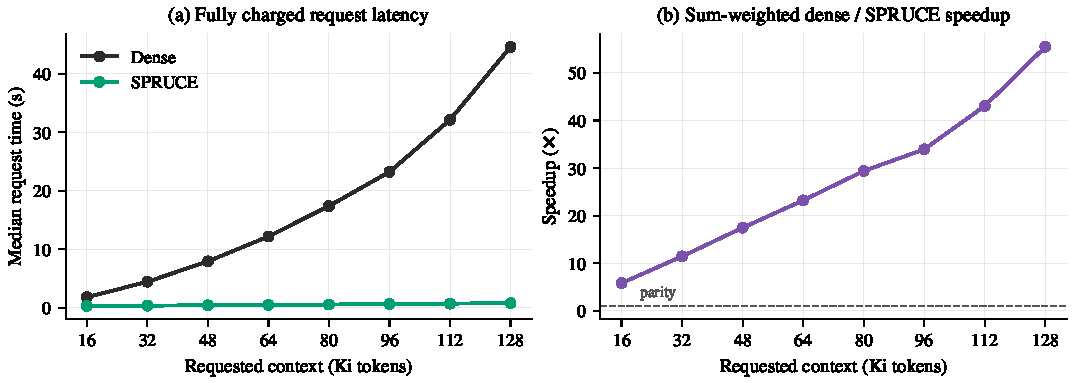
\includegraphics[width=\textwidth]{figures/fig_latency_speedup.pdf}}
\caption{Fully charged request cost, 36 prompts per length; every preprocessing,
selection, stitching, transfer, prefill, and decode cost of both arms is inside these
numbers. (a) Median request latency; dense grows superlinearly from 0.586 s at 16K
to 10.709 s at 128K, while the compiled path rises only from 0.230 s to 0.767 s.
(b) The resulting sum-weighted speedup, above parity at every length and widening
with context because compiled packet size is set by $M$ and the expansion radius,
not by the prompt.}
\label{fig:speedup}
\end{figure*}

\begin{figure*}[t]
\centerline{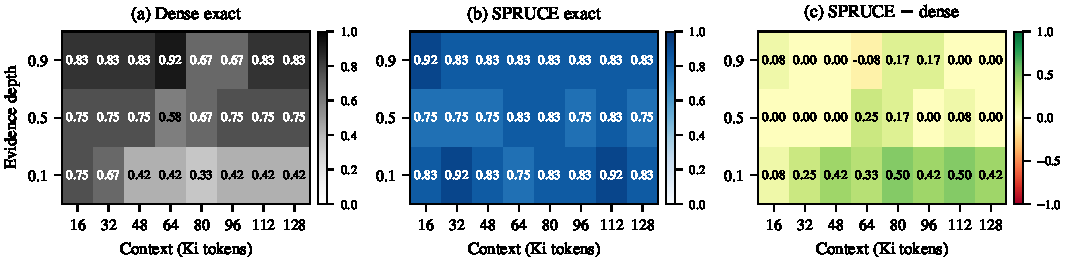
\includegraphics[width=\textwidth]{figures/fig_heatmap.pdf}}
\caption{Exact accuracy by context length and evidence depth (fraction of the
document before the evidence; 0.1 is farthest from the final question). Dense
accuracy collapses along the depth-0.1 row as length grows, reaching 0.33 at 80K,
while the compiled path stays between 0.75 and 0.92 across that row. Panel (c)
shows the gain is concentrated where dense reading is weakest;
the single negative cell is $-0.08$.}
\label{fig:heatmap}
\end{figure*}

\section{Results}
\label{sec:results}

\subsection{Accuracy}

Over the 288 paired prompts the dense model answered 192 correctly (66.667 percent,
Wilson 95 percent interval 61.03--71.86) and the compiled path 237
(82.292 percent, Wilson 77.47--86.27), an improvement of 15.625 points. Paired
outcomes were 174 both correct, 63 compiler-only, 18 dense-only, and 33 neither,
giving an exact McNemar $p=5.20\times10^{-7}$.

The compiled path was more accurate at every one of the eight tested lengths
(Table~\ref{tab2}). The two arms move in opposite directions with length: dense
falls to 55.6 percent at 80K, while compiled stays within a 5.5 point band. Over
the five lengths at 64K and above,
dense scored 113/180 (62.78 percent) against compiled 148/180 (82.22 percent), a
19.44 point gap with 47 compiler-only against 12 dense-only rows
($p=5.13\times10^{-6}$).

\begin{table}[t]
\caption{Paired results by requested context length ($n=36$ per row)}
\begin{center}
\renewcommand{\arraystretch}{1.05}
\begin{tabular}{|c|c|c|c|c|c|}
\hline
\textbf{Length} & \textbf{Dense} & \textbf{SPRUCE} & \textbf{Delta} & \textbf{Comp.-only /} & \textbf{Speed-} \\
\textbf{(Ki)} & \textbf{(\%)} & \textbf{(\%)} & \textbf{(pt)} & \textbf{dense-only} & \textbf{up} \\
\hline
16  & 77.8 & 83.3 & $+5.6$  & 4 / 2  & 2.49$\times$ \\
32  & 75.0 & 83.3 & $+8.3$  & 5 / 2  & 4.11$\times$ \\
48  & 66.7 & 80.6 & $+13.9$ & 7 / 2  & 5.78$\times$ \\
64  & 63.9 & 80.6 & $+16.7$ & 8 / 2  & 7.42$\times$ \\
80  & 55.6 & 83.3 & $+27.8$ & 12 / 2 & 9.18$\times$ \\
96  & 61.1 & 80.6 & $+19.4$ & 10 / 3 & 10.62$\times$ \\
112 & 66.7 & 86.1 & $+19.4$ & 9 / 2  & 12.43$\times$ \\
128 & 66.7 & 80.6 & $+13.9$ & 8 / 3  & 14.08$\times$ \\
\hline
\textbf{All} & \textbf{66.7} & \textbf{82.3} & $\mathbf{+15.6}$ & \textbf{63 / 18} & \textbf{9.58}$\boldsymbol{\times}$ \\
\hline
\multicolumn{6}{l}{Speedup is fully charged: dense request time divided by compiled}\\
\multicolumn{6}{l}{request time, summed per-case medians, all preprocessing included.}
\end{tabular}
\label{tab2}
\end{center}
\end{table}

\subsection{Distance from evidence to query}

The strongest effect is positional. At depth 0.1, where the evidence is farthest
from the final question, dense
scored 46/96 (47.92 percent) against compiled 81/96 (84.38 percent), a 36.46 point
gap with 40 compiler-only against 5 dense-only rows ($p=7.88\times10^{-8}$).
Restricting further to depth 0.1 at 64K and above, dense scored 24/60
(40.0 percent) against compiled 50/60 (83.33 percent), a 43.33 point gap. At depths
0.5 and 0.9 the deltas were much smaller: $+6.25$ and $+4.17$ points.

Fig.~\ref{fig:heatmap} shows this directly: the dense panel is a gradient, its
depth-0.1 row falling to 0.33 at 80K while its depth-0.9 row stays near 0.83, and the
compiled panel is close to flat. Compilation removes the positional dependence,
because afterward the evidence is always a few hundred tokens from the question.

\subsection{Efficiency and memory}

\begin{figure}[t]
\centerline{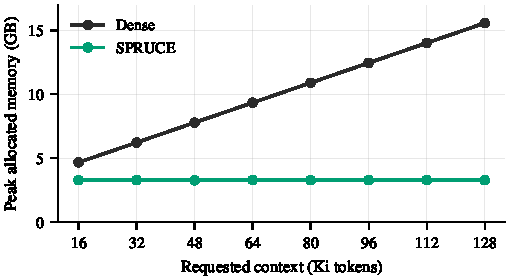
\includegraphics[width=0.90\columnwidth]{figures/fig_memory.pdf}}
\caption{Median peak \emph{allocated} GPU memory. The compiled path stays within
0.02 GB of 3.27 GB across a factor of eight in context length, while dense grows
linearly from 4.66 GB to 15.58 GB. Reserved memory is not shown: both arms alternate
in one process and PyTorch retains cached reservations, so both traces equal the
dense high-water mark.}
\label{fig:memory}
\end{figure}

\begin{figure}[b]
\centerline{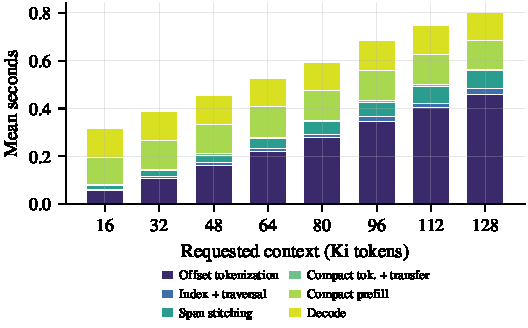
\includegraphics[width=0.88\columnwidth]{figures/fig_compiled_latency.pdf}}
\caption{Mean fully charged request components for the compiled path. Selection is
the thin band barely visible; traversal averages 2.344 ms. Offset tokenization is the
only stage that scales with context.}
\label{fig:latency}
\end{figure}

The compiled path was faster at every length with all preprocessing charged
(Fig.~\ref{fig:speedup}): only the dense arm carries a quadratic term over the full
document. Summed per-case median request time was 1,368.499 s dense against
142.836 s compiled, a 9.581 times sum-weighted speedup, with per-length values from
2.49 to 14.08 times and a median per-prompt speedup of 8.29 times (IQR
4.97--11.54). The median model-prefill component alone was 3.732 s against
0.039 s.

Median compiled input was 1,849.5 tokens, 2.46 percent of the original prompt; at
128K it was 1,842.5 tokens, 1.41 percent. Packet size is fixed by $M$ and the radius, not
the prompt, so the retained fraction falls as the document grows, which is why
Fig.~\ref{fig:speedup}b rises roughly linearly rather than flattening.

The compiler's own cost is small but not zero, and its distribution is informative
(Fig.~\ref{fig:latency}): mean compiled request components sum to 0.4945 s, of which
full-prompt tokenization is 53.90 percent, dense decode 24.54 percent, span stitching
9.77 percent, compact prefill 7.78 percent, hierarchy construction 2.37 percent, and
tree selection only 0.47 percent (2.344 ms). The dominant remaining cost is offset
tokenization, a CPU cost rather than an attention cost.

Memory behaves as the token counts predict (Fig.~\ref{fig:memory}). Median peak
allocated GPU memory was 4.658 GB dense against 3.269 GB compiled at 16K, and
15.582 GB against 3.273 GB at 128K, a 79.0 percent reduction. The residual 3.27 GB is
almost entirely FP16 backbone weights. We report allocated memory only: reserved memory is not comparable, since the arms
alternate in one process and the allocator retains reservations.

\subsection{Where the remaining errors come from}

Because SPRUCE physically removes text, its failures are separable: either the
evidence reached the packet or it did not.
Direct $M=4$ recall was 232/288 and radius-1 expansion raised it to 256/288
(88.89 percent), repairing 24 direct misses, 21 of which became exact.

With the expanded evidence present, compiled
accuracy was 237/256 (92.58 percent) and all 63 compiler-only wins fall here with zero
dense-only losses; without it, accuracy was 0/32 and all 18 dense-only losses fall
here, each a selection miss, not a reading failure.

Two cases fail for reasons unrelated to routing: the civic case
(\texttt{council\_vote19\_6}) scored 0/24 in \emph{both} arms with the evidence
present, and the astronomy case (\texttt{polaris\_field508}) had full recall but
scored 17/24 on near-misses. The principal selector failure is the engineering case
(\texttt{alloy\_r62}), at 4/24 against 22/24 dense with expanded recall of only
4/24 --- a lexical sketch cannot separate affirmative evidence from a similar negated
distractor.

\subsection{Scope of the claim}

Eight of the 12 semantic cases show a positive delta, three tie, one
(\texttt{alloy\_r62}) is negative. A seeded 10,000-draw bootstrap clustered by
semantic case has a median of $+15.625$ points but a 95 percent interval of
$[-5.556, +34.722]$ that crosses zero: the 288 rows are repeated observations from
12 clusters, not independent tasks.

\section{Conclusion}

Long context is now standard, and most work treats what remains as a cost problem
inside the model, selecting inside attention and measuring against dense
reading. Our results indicate dense attention
was not the ceiling in accuracy: with the whole document in view a frozen
Qwen2.5-Coder-1.5B answered 66.7 percent of the sealed suite, falling to 40.0 percent
where the evidence sat farthest from the question.

Compiling those same documents to a median 1,849.5 tokens of exact source text
raised accuracy to 82.3 percent, with the gain largest where dense reading was
weakest. Because that packet is sized by the selection budget rather than the prompt,
the model's input, prefill and KV cache are all independent of context length: the
request is linear in it, 9.58 times faster, at flat memory.

We do not claim general superiority over dense reading. SPRUCE loses access to
omitted information, but on this retrieval suite, focusing the model on selected
exact evidence produced substantially higher accuracy than full dense reading.
Establishing more requires external benchmarks such as LongBench, RULER and
InfiniteBench, larger and non-Qwen backbones, and head-to-head comparison with the
methods above. We report a paradigm and one controlled result, not a benchmark
claim. The lexical pass is one optimization among many: dead-context elimination and structural, table-aware or code-aware passes all fit the
same frame.

\begin{thebibliography}{00}
\bibitem{hip} H. Lee \textit{et al.}, ``A training-free sub-quadratic cost transformer model serving framework with hierarchically pruned attention,'' in \textit{Proc. Int. Conf. Learn. Represent. (ICLR)}, 2025, arXiv:2406.09827.
\bibitem{seer} Y. Gao \textit{et al.}, ``SeerAttention: Learning intrinsic sparse attention in your LLMs,'' arXiv preprint arXiv:2410.13276, 2024.
\bibitem{spot} H. Ahmad and S.-Y. Yun, ``SpotAttention: Plug-in block-sparse routing for pretrained long-context transformers,'' arXiv preprint arXiv:2606.22874, 2026.
\bibitem{hisa} Y. Xu \textit{et al.}, ``HISA: Efficient hierarchical indexing for fine-grained sparse attention,'' arXiv preprint arXiv:2603.28458, 2026.
\bibitem{dsa} DeepSeek-AI, ``DeepSeek-V3.2: Pushing the frontier of open large language models,'' arXiv preprint arXiv:2512.02556, 2025.
\bibitem{misa} R. Zhou, F. Meng, Y. Xu, T. Liu, G. Lu, M. Zhang, and W. Pei, ``MISA: Mixture of indexer sparse attention for long-context LLM inference,'' arXiv preprint arXiv:2605.07363, 2026.
\bibitem{seerr} Y. Gao \textit{et al.}, ``SeerAttention-R: Sparse attention adaptation for long reasoning,'' arXiv preprint arXiv:2506.08889, 2025.
\bibitem{quoka} D. Jones, J. Park, M. Morse, M. Lee, C. Lott, and H. Langston, ``QUOKA: Query-oriented KV selection for efficient LLM prefill,'' arXiv preprint arXiv:2602.08722, 2026.
\bibitem{qwen} B. Hui \textit{et al.}, ``Qwen2.5-Coder technical report,'' arXiv preprint arXiv:2409.12186, 2024.
\bibitem{yarn} B. Peng, J. Quesnelle, H. Fan, and E. Shippole, ``YaRN: Efficient context window extension of large language models,'' arXiv preprint arXiv:2309.00071, 2023.
\end{thebibliography}

\end{document}